
\subsubsection*{Coupling a static root system to DuMux} \label{sec:dumux_coupling}

Putting the sections \ref{ss:mapping} and \ref{ssec:xylem} together, we can easily set up an example, using the classic sink term in the soil model, similar as in \citep{leitner2014impact} based on \citep{doussan1998modelling}. For solving the Richards equation we use DuMux \citep{koch2020dumux}.

The next example mimics benchmark C12 \citep{schnepf2019call}, but with a static simulated root system. The example must be run out of dumux-rosi (located in dumux-rosi/rosi$\_$benchmarking/python$\_$solver/coupled), otherwise the DuMux Python coupling is not available. 

\lstinputlisting[firstline=1, language=Python, caption=Example 6c]{examples/example6c_coupling.py}

\begin{itemize}
\item[3,4] Add paths for DuMux Python coupling (L3) and Python solvers (L4).

\item[5,6] The direct C++ part of the DuMux binding, and the Python wrapper class. 

\item[17,18]  Defines a sinusoidal function for the collar boundary condition.

\item[21-37] All parameters that are needed for this simulation. L25 decides if periodic boundary conditions are used, or not. L35 states the simulation time, L36 the initial root system age. L37 defines if age dependent root conductivities are used. The rooot conductivities are hard coded in the file root\_conductivities.py, that is imported in L8. Age dependent conductities can be used to mimic root growth in a predefined way, i.e. the root system is already fully grown, but the radial conductivities are turned on during the simulation. 

\item[41-49] Sets up the soil solver (DuMux Python binding from dumux-rosi). 

\item[52-62] Sets up the Xylem model as in Subsection \ref{ssec:xylem}. If the root system is not periodic, a confining geometry is set L54-L58. L62 passes the axial and radial conductivities to the XylemFluxPython object (the function is defined in root\_conductivities.py).

\item[65-70] Coupling between the soil soil and root part is performed by setting the picking function that assigns a cell index to each spatial position L65, and L66. In L67 root segments are cut to the rectangular grid, and in L70 the cell index of the root collar is determined. 

\item[73-77] Initializes the simulation, initially the soil values are the same as the initial conditions (L75).

\item[79-94] First, we calculate the xylem matric potential $rx$ for a given soil matric potential $sx$ (L81) and save the actual collar flux for later analysis (L83). Next, we calculate teh sink (L85) and apply it to the soil model (L86). The soil model is simulated (L87) and the resulting matric potential $sx$ is updated (L88). The simulation takes some time (around 15 minutes), and L90-93 print debugging information and a progress bar. L94 increases the current simulation time. This is needed if age dependent conductivities are used. 

\item[99-111] L99 creates Figure \ref{fig:example6c} and, L102-111 plots uptake and cumulative uptake over time, see Figure \ref{fig:uptake}.
\end{itemize}

\subsubsection*{Coupling a dynamic root system to DuMux with soil feedback} \label{sec:dumux_dyn_coupling}

We modify Example \ref{sec:dumux_coupling}. Using the class MappedRootSystem (as before) it is sufficient to call MappedRootSystem::simulate() to implement real root growth, i.e. to add rs.simulate(dt) in L80. The modified segments and the mapping of new segments is automatically managed (see example7b\_coupling.py). Figure \ref{fig:example7c} shows the root actual uptake over time, with a slightly altered shape compared to \ref{fig:example6c}. Note that the jumps in actual uptake are due to emerging root segments.

In this example soil state does not affect root system growth in any way. We need to add the processes we are interested in (see Section \ref{sec:tropism} and \ref{sec:functional}). For demonstration how to do that, we demonstrate the implementation steps using hydrotropim. Note that the other interactions from Section \ref{sec:functional} could be implemented in the same way. 

In order to use hydrotropism, we need to define a SoilLookUp that accesses the dynamic soil data. We present two approaches: the first uses nearest neighbour interpolation, which is fast but a coarse approximation. The second uses linear interpolation which is more exact, but slower. 

\lstinputlisting[firstline=1, language=Python, caption=Example 7c]{examples/example7c_feedback.py}

We only describe the changes to Section \label{sec:dumux_coupling}:

\begin{itemize}
\item[18-25] We first create a class for nearest neighbour interpolation that extends pb.SoilLookUp. L22 stores a reference to the DuMux soil model. For specialisation of pb.SoilLookUp we need to overwrite the getValue function (L24-25). First we retrieve the cell index by calling $pick$. And, then we return the solution at this cell (in Pascal). Note that the solution is the same for each point within a cell. 
\item[28-41] Secondly, we want to use linear interpolation, which is slower, but more exact. The constructor stores a reference to the soil model (L30-34) the coordinates of the degrees of freedom (i.e. where the points where numerical solution is defined) and calls update(), which fetches the current model solution. Update will be called in after each solving step in the simulation loop. L39-L41 performs the linear interpolation. This is rather slow because the method assumes an unstructured grid, and is not optimized for a structured rectangular grid. 
\item[94-100] We set tropism to hydrotropism (L98) and modify the tropism parameters (L99,100)
\item[102,103] We set the soil, using nearest neighbour or linear interpolation.
\item[120,121] If we use linear interpolation we need to call update to copy the current solution. 
\item[122] Root system simulation, updates geometry and mappers.
\end{itemize}

Figure \ref{fig:example7c} shows that hydrotropism will lead to increased cumulative uptake, because the roots are more evenly distributed. Note that there is a big variation in the results, and for a more profound analysis we would have to make many simulation runs. 

% \begin{figure}
% \begin{subfigure}[c]{1\textwidth}
% 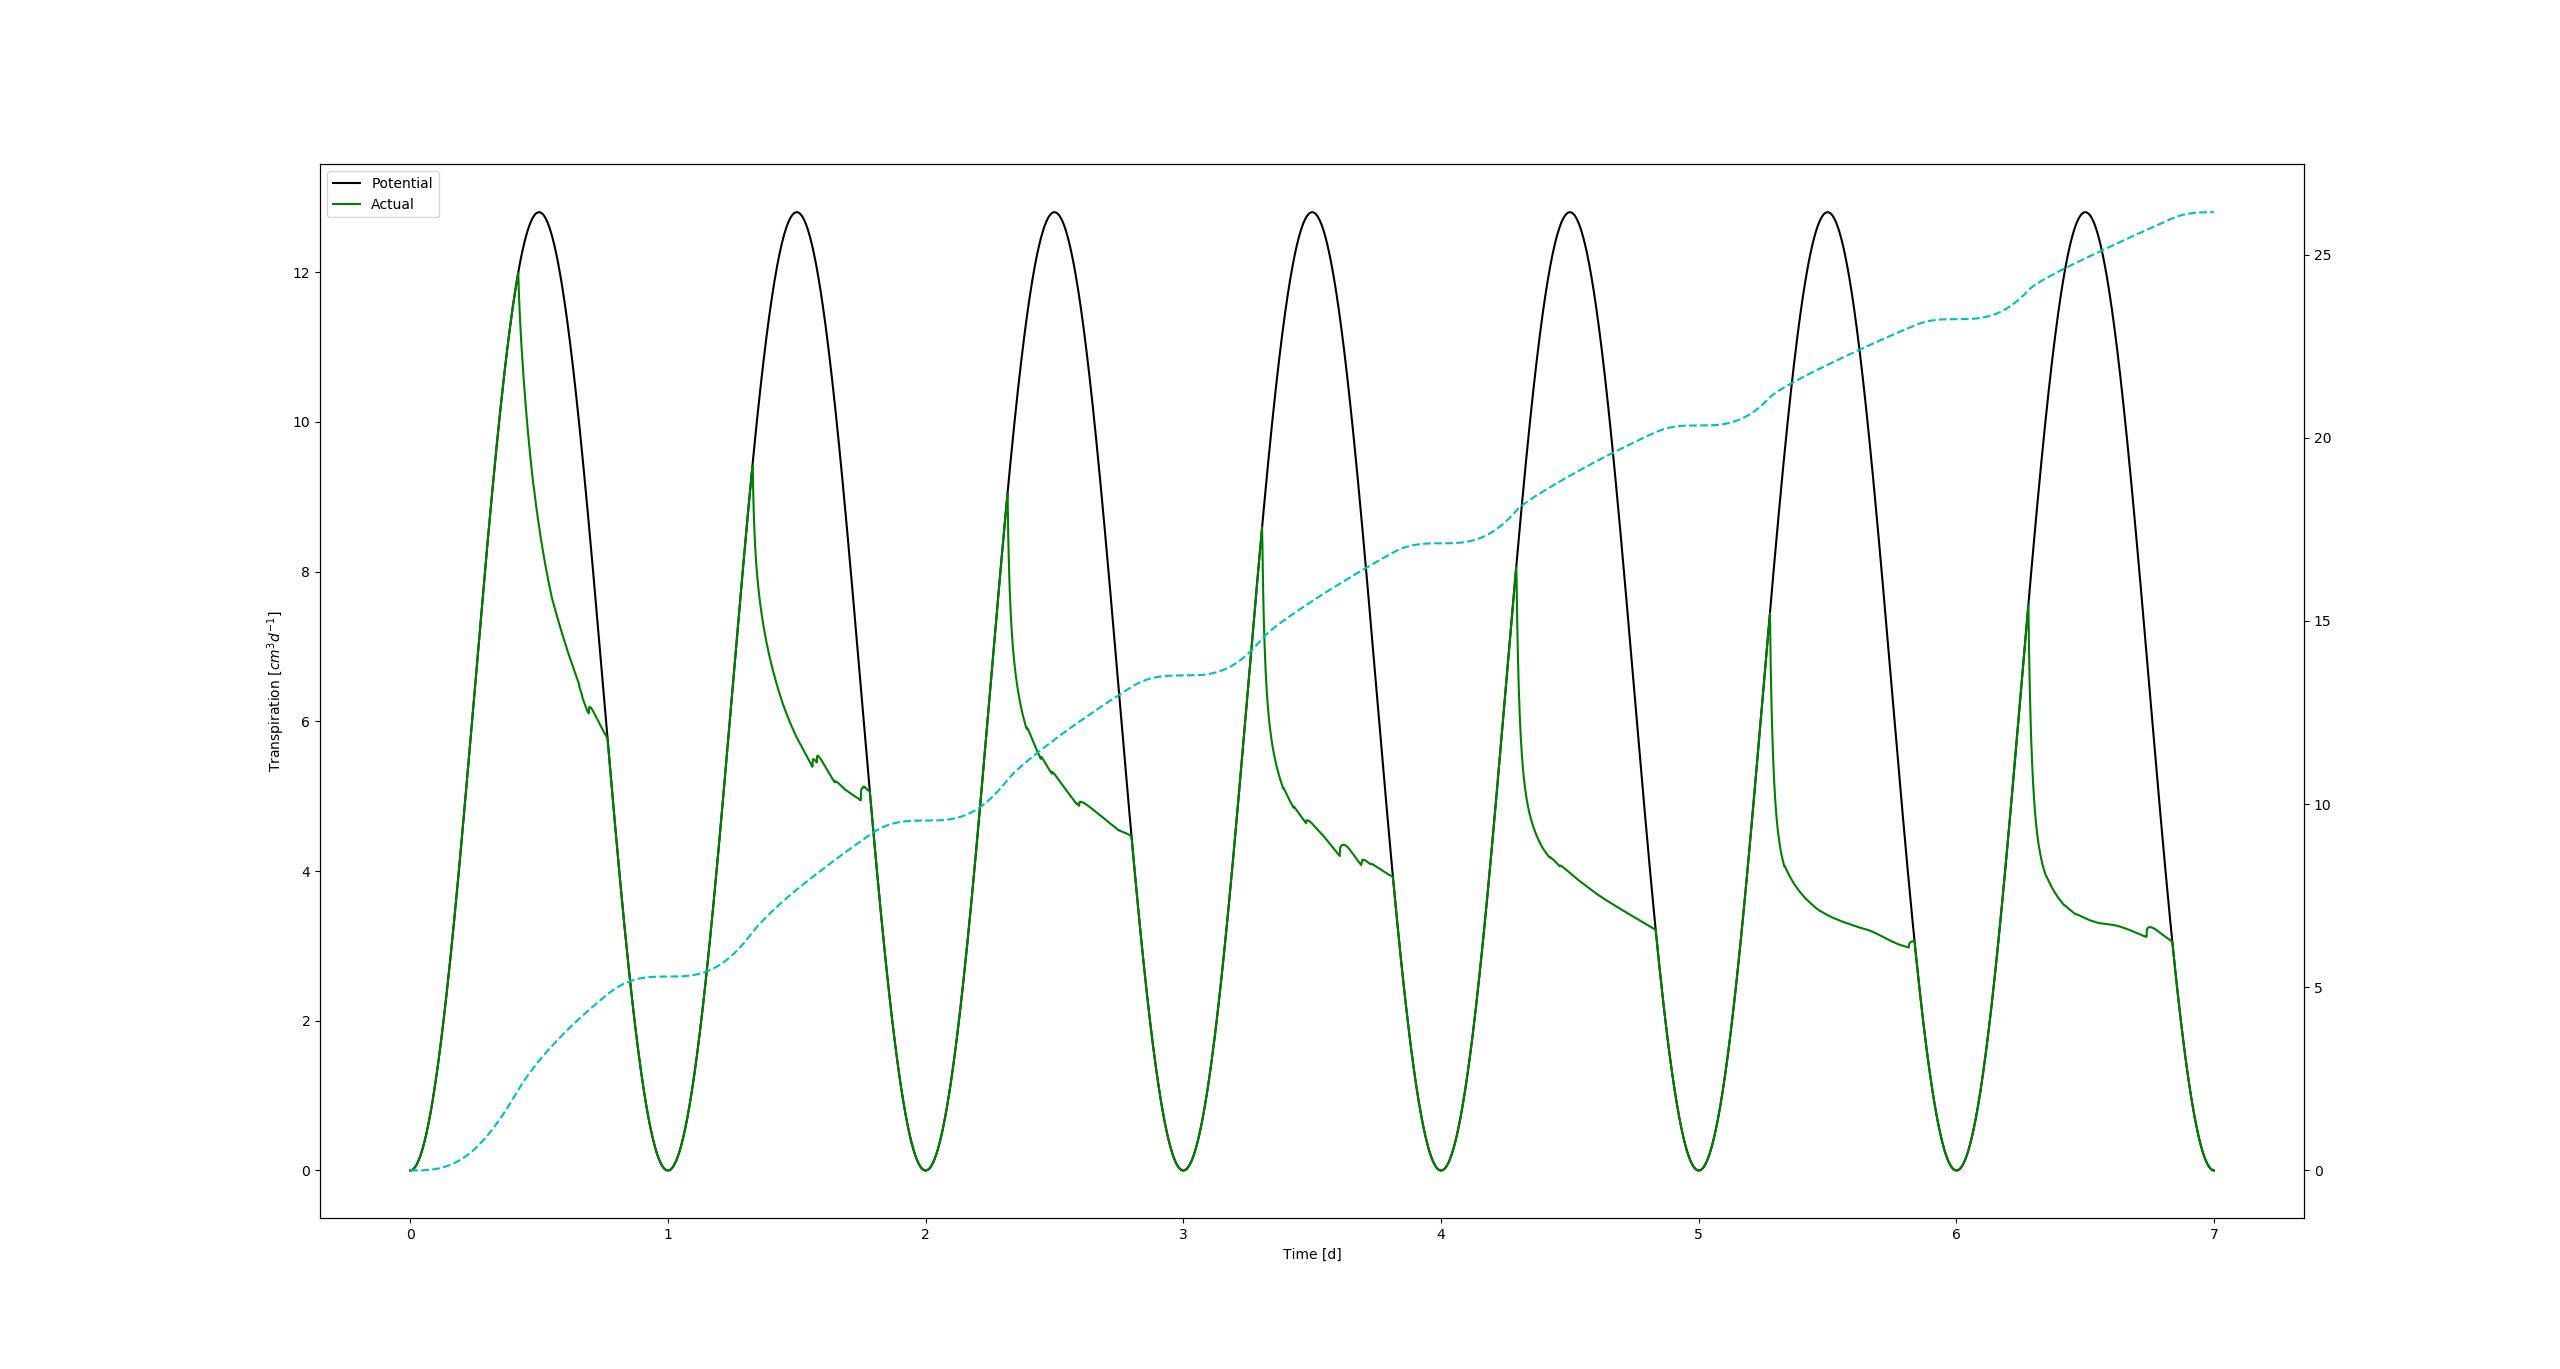
\includegraphics[width=0.99\textwidth]{example7c_no_hydro.png}
% \subcaption{Gravi- and Plagiotropism} \label{fig:example7c}
% \end{subfigure}
% \begin{subfigure}[c]{1\textwidth}
% 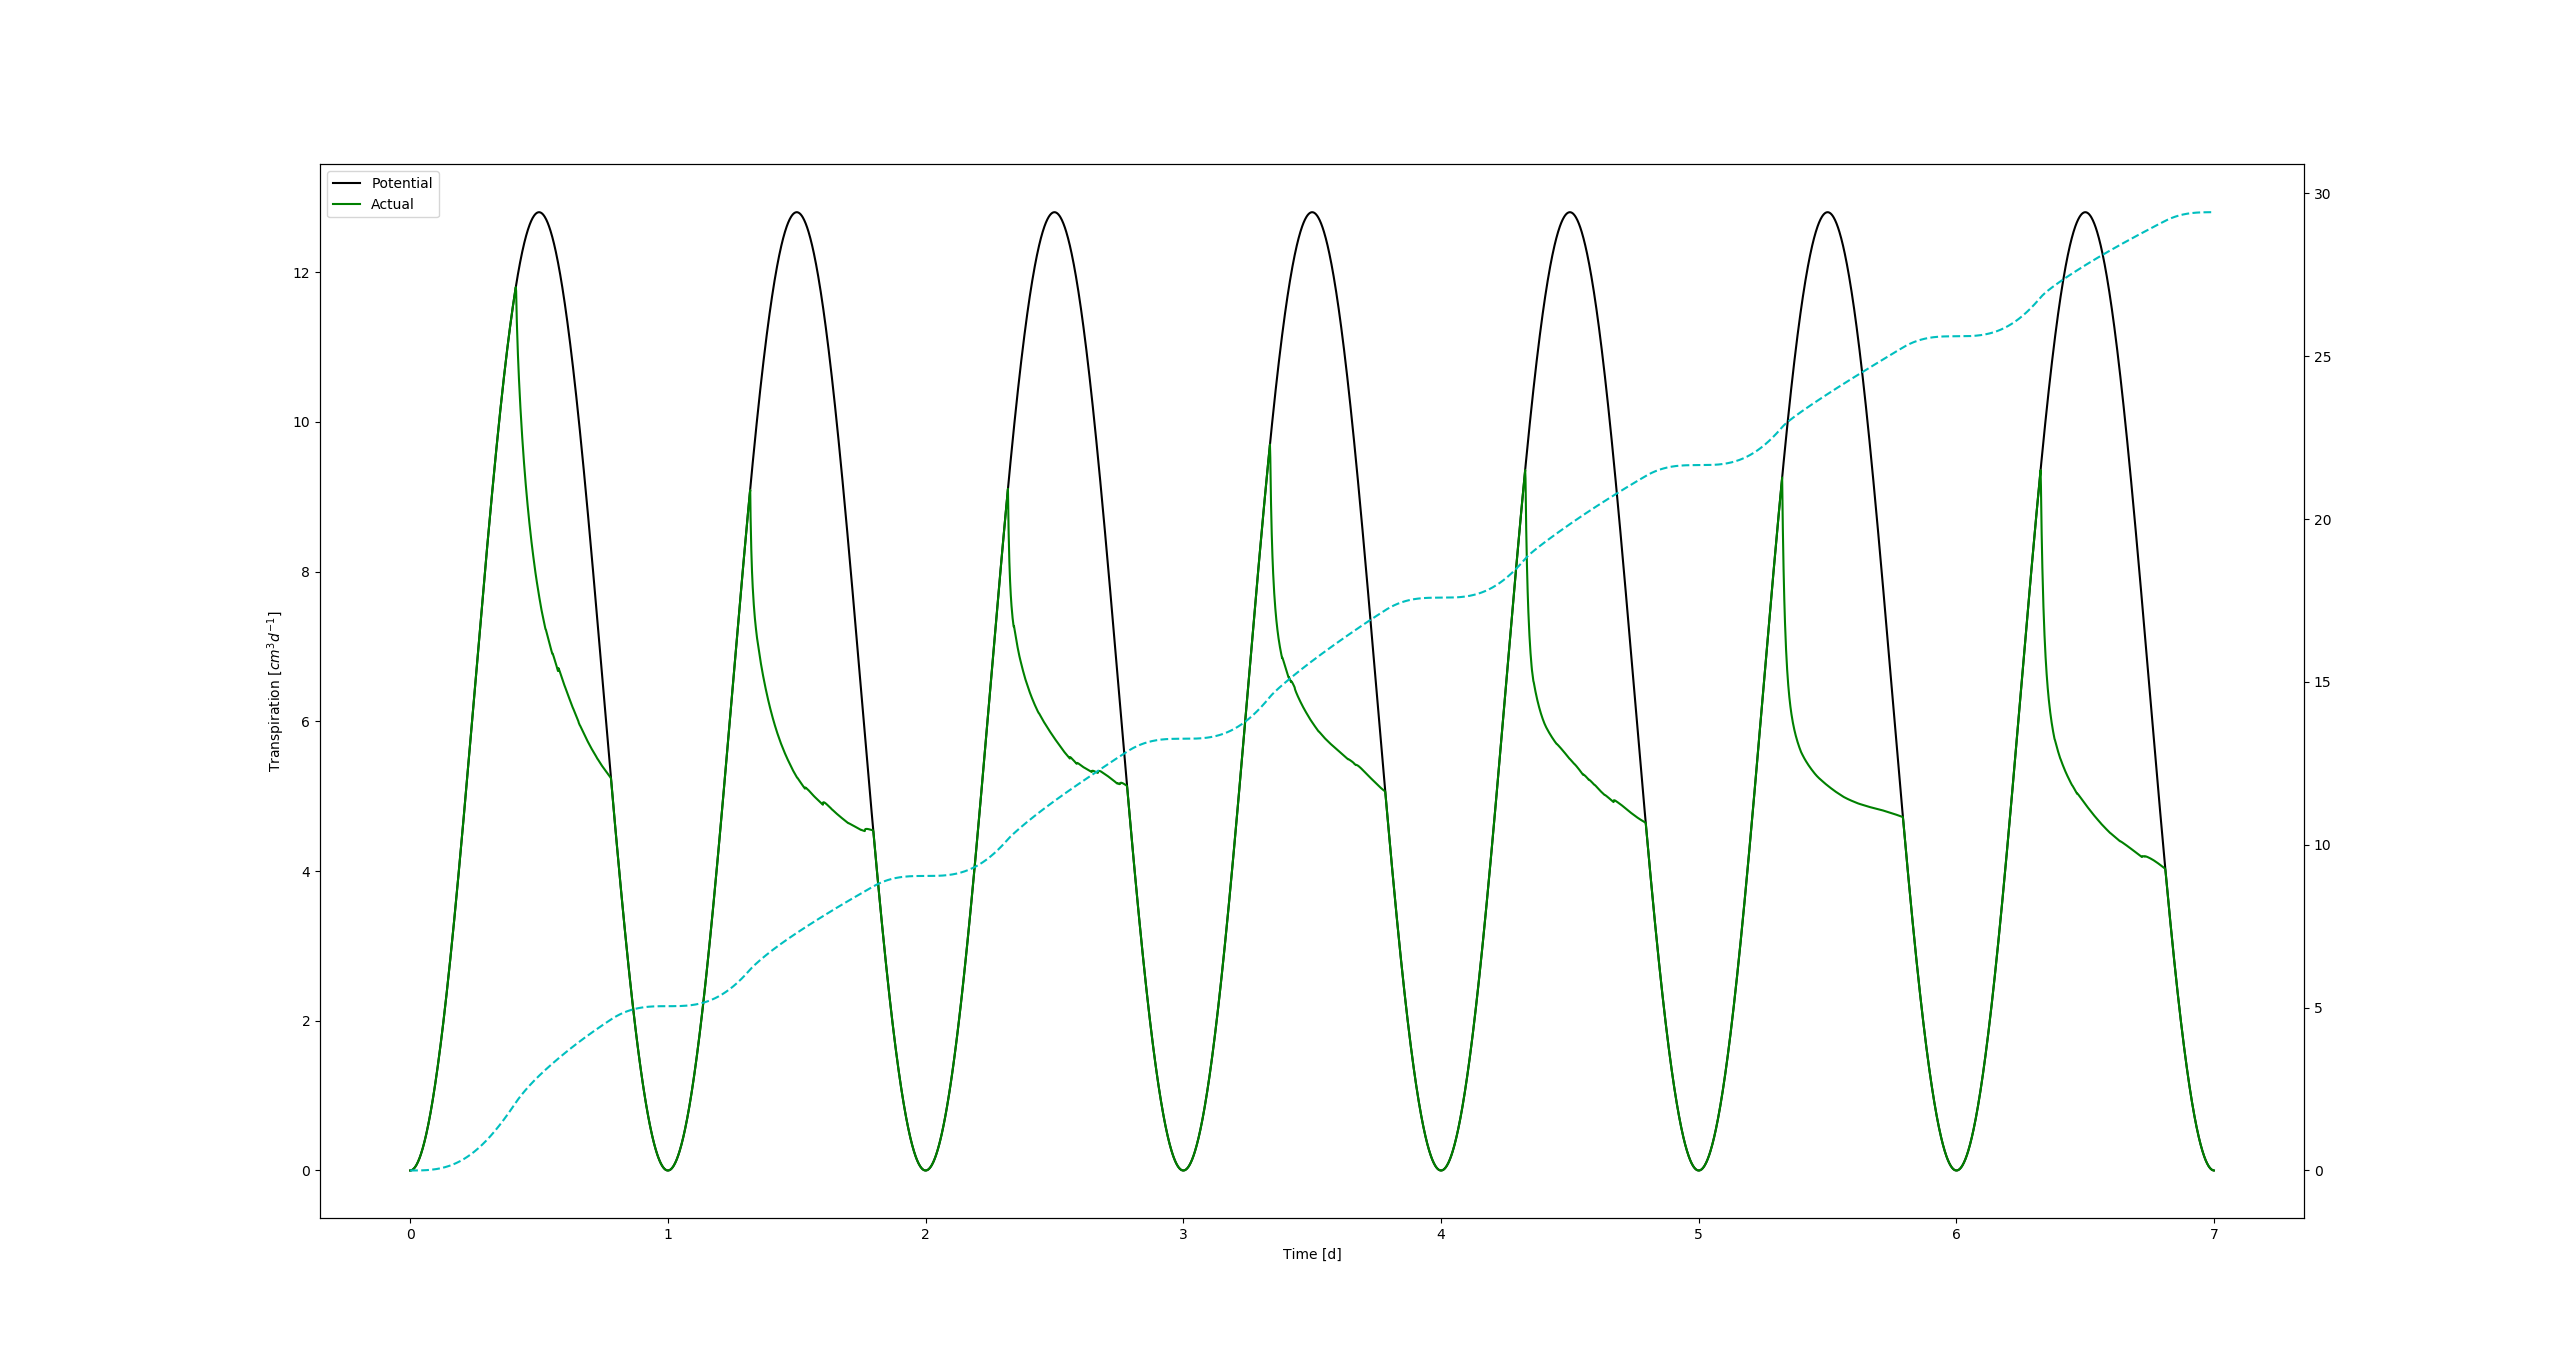
\includegraphics[width=0.99\textwidth]{example7c_simple_hydro.png}
% \subcaption{Hydrotropism} \label{fig:example7c_hydro}
% \end{subfigure}
% \caption{Water uptake a in plant pot} \label{fig:example7c}
% \end{figure}



\subsubsection*{Mimicking root growth}

For a pre-grown root architecture, root growth can be mimicked in a dynamic soil-root interactions simulation using the creation times of the root segments. The root axial conductence $k_x$ is set equal to 0 for ``unborne" root segments with negative age. The root radial conductivity, $k_r$ needs to be equal to 0 (not just a small value) for segments with negative  age. 
The parameter \lstinline{initialT} should be equal to 1 if one wants to mimic growth and equal to the final simulation time if not. 
With respect to solute transport, the diffusion coefficient needs to be very small  for unborn segments (?).



\subsubsection*{Estimating the hydraulic conductivity drop in the rhizosphere} \label{sec:hydro_rhizo}

The resolution of the soil grid is often too coarse to catch small-scale rhizosphere gradients in hydraulic conductivity near the roots. The consequence is that root water uptake is overestimated. One solution would be (adaptive) grid refinement, however at the cost of computation time and the validity of the line-source assumption that we take for the roots in our setup. 
An alternative solution is to keep the coarse soil grid resolution and estimate the soil water potential at the root-soil interface. We implemented two ways of doing so within dumux-rosi. Firstly, we split the volume of each soil control element between the root segments that lie inside it, and assign a soil cylinder around each root segment. In each soil cylinder, the 1D radially symmetric Richards equation is solved and coupled to the macroscopic scale in a mass conservative way via the outer boundary conditions of the soil cylinders. 

Another approach is described in this example and follows the approach described in \cite{Schroeder2008}. Each root segment inside a soil control element of volume $V_s$ has an assigned ``rhizosphere soil volume" equal to $$V_{rhizo} = k V_s,$$ where the weighting factor $k$ is the fraction of the root segment volume $V_{rs}$ relative to the overall volume of roots $V_{rst\textsc{}}$ inside $V_s$, $k=\frac{V_{rs}}{V{rst}}$. 
From this, the outer radius of the rhizosphere cylinder is computed by 
$$r_{out}=\sqrt{\frac{V_{rhizo}+V_{rs}}{\pi l}},$$ where $l$ is the root segment length. 


Then the flux at the root-soil interface is estimated based on the analytical solutions of the 1D radially symmetric Richards equation. Based on the steady-rate assumption and using the matric flux potential $\Phi(h_c)=\int_{-\infty}^{h_c}  K(h) dh$ that linearizes the Richards equation, the radial matric flux potential profiles for non-stressed and stressed conditions are given by 
\begin{multline}
\Phi(r)=\Phi_{r_{out}} + (q_{root}r_{root}-q_{out}r_{out})\left[ \frac{r^2/r_{root}^2}{2(1-\rho^2)} + \frac{\rho^2}{1-\rho^2}\left(\text{ln}  \frac{r_{out}}{r}-\frac{1}{2} \right) \right] \\\ + q_{out}r_{out} \text{ln} \frac{r}{r_{out}}
\end{multline}
and 
\begin{multline}
\Phi(r) = \left(\Phi_{r_{out}} - \Phi_{r_{root}} + q_{out}r_{out}\text{ln} \frac{1}{\rho}\right)\frac{r^2/r_{root}^2 - 1 + 2\rho^2 \text{ln}  r_{root}/r}{\rho^2 -1 + 2\rho^2 ln 1/\rho} \\\ + q_{out}r_{out}\text{ln} \frac{r}{r_{root}} + \Phi_{root},
\end{multline}
where $\rho=\frac{r_{out}}{r_{root}}$, $r_{root}$ is the root radius, $r_{out}$ is the outer radius, $q_{root}$ is the flux prescribed at the root-soil interface, $q_{out}$ is the flux at the outer boundary.

Given the soil matric potential at the outer boundary, and either the flux (non-stressed conditions) or soil matric potential (stressed) at the root-soil interface, the solution computes the radial matrix flux potential profile, and from the matric flux potential, the soil matric potential can be inferred. The soil matric potential at the outer boundary is taken to be the macroscopic soil matric potential value of the given soil control element at the given time step. The water flux at the outer boundary, $q_{out}$, is computed such that the sum of the fluxes at the outer boundaries of the rhizosphere cylinders is equal to the net flux into or out of the given soil control element, $q_{V_s}$, at a given time step, and $$q_{out}=k q_{V_s}$$, where $k$ is the same weighting factor as described above. However, setting the outer flux to zero is sufficient in most cases, as there is redistribution after every time step.  

We start the simulation by computing the root water uptake according to the classical (see section \ref{s:coupling}). 
Then, for every root segment and at every time step, we check whether the matric flux potential at the root-soil interface is positive or negative. In case the matric flux potential is positive, root water uptake follows non-stressed conditions, and the sink term is left according to the classical approach. In case the matric flux potential is negative, root water uptake follows stressed conditions and the soil matric potential at the root-soil interface is equal to the wilting point. The water flux from soil into the root is computed by numerically approximating the soil matric potential gradient at the root-soil interface and multiplying this by the hydraulic conductivity.

Finally, the flux at the root-soil interface is the maximum of the classical and steady-rate approximation value. This makes sure that hydraulic redistribution (i.e. flow from roots to soil) is still possible. 

Listing X shows the code of file ``coupled\_c12\_schroeder.py".
%\lstinputlisting[firstline=1, language=Python, caption=Example 6a]{../examples/example6a_mapping.py}

\begin{itemize}
\item[106-110] Root xylem potentials are computed based on the current soil (at first call) or rhizosphere (from second call onwards) water potentials. 
\item[112] Rhizosphere soil water potentials are updated from the current soil and xylem water potentials using the steady-rate assumption. 
\item[113] For each root segment, the water fluxes are computed from the current xylem and rhizosphere water potentials. 
\item[115] For the soil control element, sum of root water uptake over all root segments inside a given soil control element is computed. 
\item[127] The fluxes are set as sources in the soil problem (Richards equation)
\item[131] Soil problem is solved for one time step. 
\end{itemize}

   
Listing Y shows the C++ code for the computation of matric potential at the root-soil interface according to \citep{Schroeder2008}. The fluxes are then computed according to the pressure differences...
%\lstinputlisting[firstline=1, language=Python, caption=Example 6a]{../examples/example6a_mapping.py}

\begin{itemize}
\item[234] Computation of the matrix flux potential according to the non-stressed equation. 
\item[237] For positive mfp (no stress), the soil matric potential at the root-soil interface is set to the corresponding value.
\item[240] For negative mfp (stress), the soil matric potential at the root-soil interface is set equal to the wilting point. 
\item[245] If the xylem water potential is larger than the root-soil interface potential, root-soil interface potential is set equal to the xylem water potential (no flux). 
\item[248] On the macroscopic scale, flow of water from root to soil is enabled. 
\end{itemize}


Figure \ref{fig:schroeder} the transpiration rate and cumulative transpiration computed based on the steady-rate assumption for the case of a clay soil. 

% \begin{figure}
% %\begin{subfigure}[c]{1\textwidth}
% 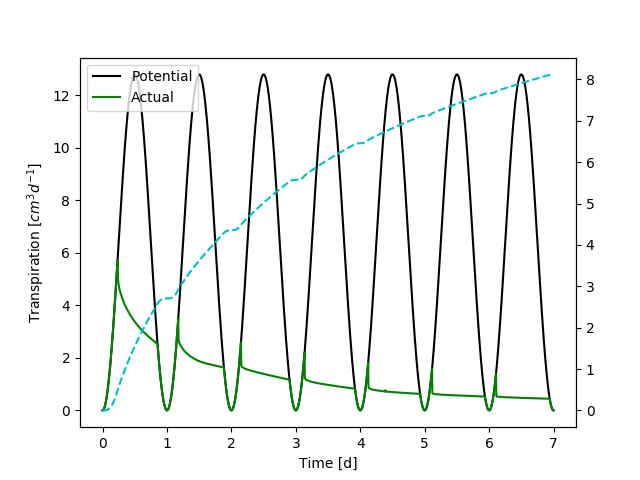
\includegraphics[width=0.99\textwidth]{clay_schroeder.png}
% %\subcaption{Gravi- and Plagiotropism} \label{fig:example7c}
% %\end{subfigure}
% %\begin{subfigure}[c]{1\textwidth}
% %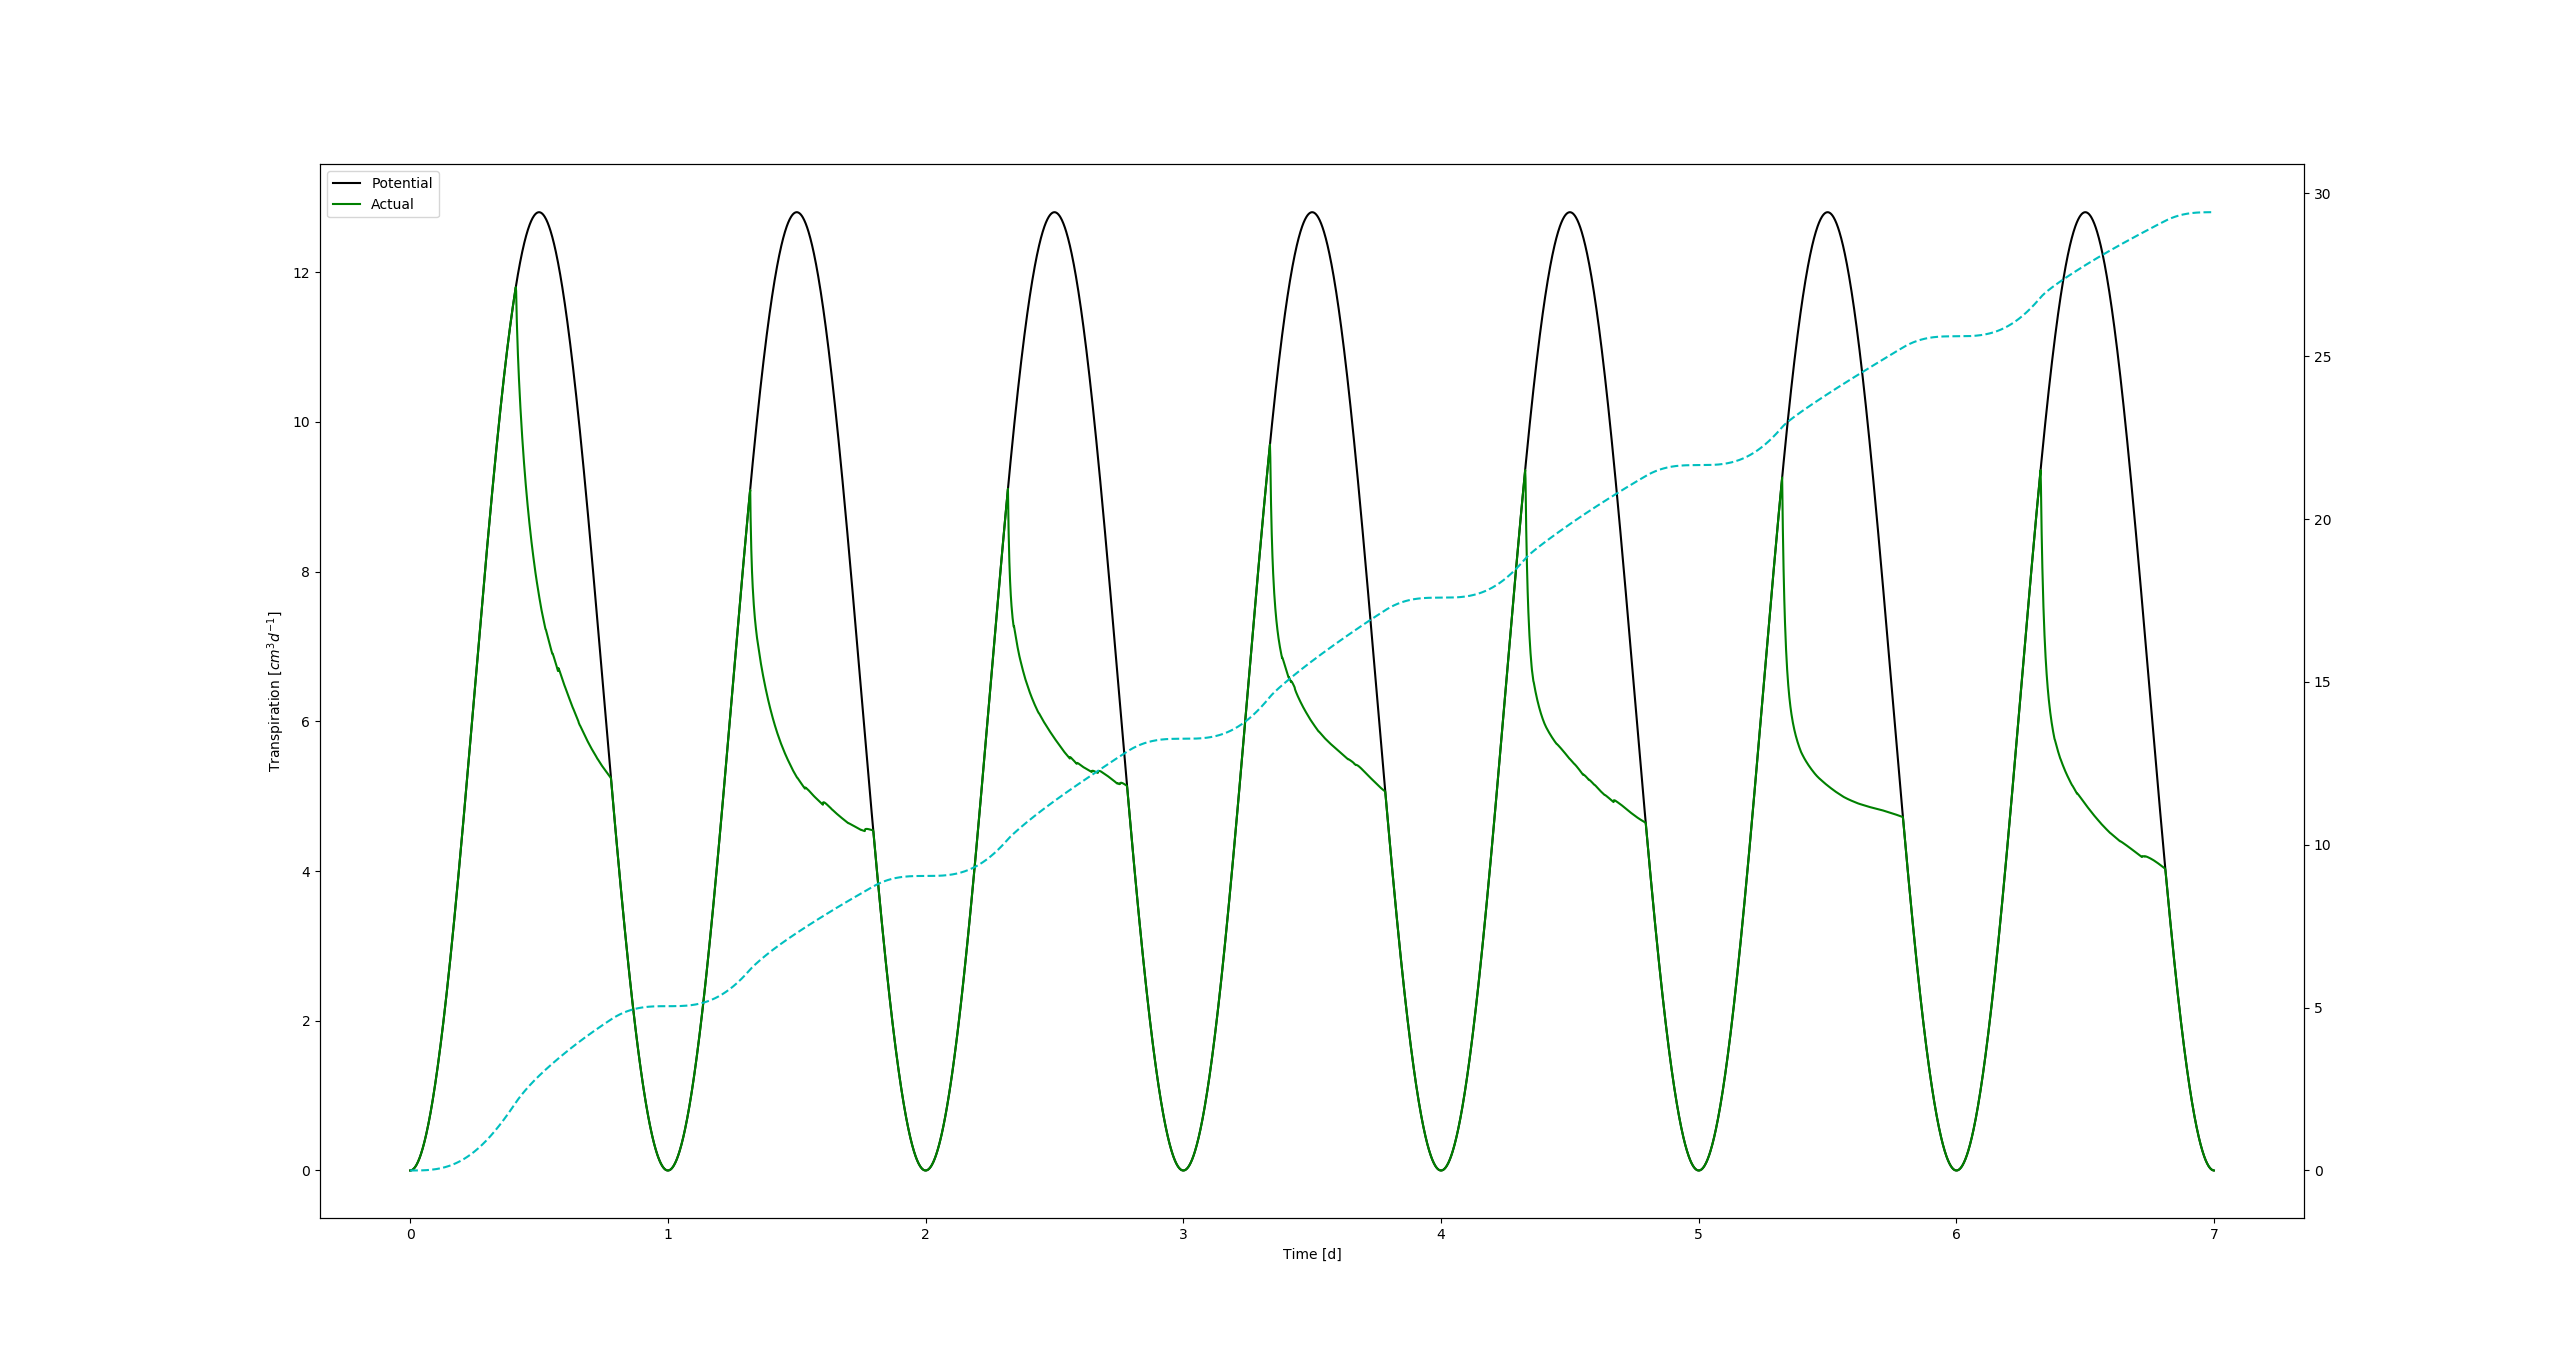
\includegraphics[width=0.99\textwidth]{example7c_simple_hydro.png}
% %\subcaption{Hydrotropism} \label{fig:example7c_hydro}
% %\end{subfigure}
% \caption{Transpiration rate and cumulative transpiration computed based on the steady-rate assumption.} \label{fig:schroeder}
% \end{figure}






